\let\negmedspace\undefined
\let\negthickspace\undefined
\documentclass[journal]{IEEEtran}
\usepackage[a5paper, margin=10mm, onecolumn]{geometry}
%\usepackage{lmodern} % Ensure lmodern is loaded for pdflatex
\usepackage{tfrupee} % Include tfrupee package

\setlength{\headheight}{1cm} % Set the height of the header box
\setlength{\headsep}{0mm}     % Set the distance between the header box and the top of the text

\usepackage{gvv-book}
\usepackage{gvv}
\usepackage{cite}
\usepackage{amsmath,amssymb,amsfonts,amsthm}
\usepackage{algorithmic}
\usepackage{graphicx}
\usepackage{textcomp}
\usepackage{xcolor}
\usepackage{txfonts}
\usepackage{listings}
\usepackage{enumitem}
\usepackage{mathtools}
\usepackage{gensymb}
\usepackage{comment}
\usepackage[breaklinks=true]{hyperref}
\usepackage{tkz-euclide} 
\usepackage{listings}
% \usepackage{gvv}                                        
\def\inputGnumericTable{}                                 
\usepackage[latin1]{inputenc}                                
\usepackage{color}                                            
\usepackage{array}                                            
\usepackage{longtable}                                       
\usepackage{calc}                                             
\usepackage{multirow}                                         
\usepackage{hhline}                                           
\usepackage{ifthen}
\usepackage{lscape}
\begin{document}

\bibliographystyle{IEEEtran}



\title{4.11.34}
\author{EE25BTECH11057 - Rushil Shanmukha Srinivas
}
% \maketitle
% \newpage
% \bigskip
{\let\newpage\relax\maketitle}

\renewcommand{\thefigure}{\theenumi}
\renewcommand{\thetable}{\theenumi}
\setlength{\intextsep}{10pt} % Space between text and floats

\numberwithin{equation}{enumi}
\numberwithin{figure}{enumi}
\renewcommand{\thetable}{\theenumi}
\newcommand{\absdet}[1]{\left|\det\!\left(#1\right)\right|}

\textbf{Problem:} Find the area of the region bounded by the lines 3x-2y+1=0,2x+3y-21=0 and x-5y+9=0 .

\textbf{Solution:}
Given three lines are
\begin{align}
\myvec{3 & -2}\myvec{x\\y} = -1 \Longrightarrow \vec{n}^\top\vec{x} = -1
\end{align}
\begin{align}
\myvec{2 & 3}\myvec{x\\y} = 21 \Longrightarrow \vec{m}^\top\vec{x} = 21
\end{align}
\begin{align}
\myvec{1 & -5}\myvec{x\\y} = -9 \Longrightarrow \vec{p}^\top\vec{x} = -9
\end{align}
The three lines form a triangle.
The vertices of triangle are obtained by 

\textbf{Intersection of :}
\begin{align}
\vec{n}^\top\vec{x} = -1 \ and \ \vec{m}^\top\vec{x} = 21 
\end{align}
The augmented system in matrix form is

\begin{align}
\myvec{
3 & -2 &\vrule& -1\\
2 & 3 &\vrule& 21} \xrightarrow{R_2 \longrightarrow 3R_2-2R_1}
\myvec{
3 & -2 &\vrule& -1\\
0 & 13 &\vrule& 65}
\end{align}
$ From \ the \ second \ row \ we \ get\ y=5 \ so \ x=3 \Longrightarrow
\vec{A} = \myvec{3\\5}$

\begin{align}
\vec{m}^\top\vec{x} = 21 \ and \ \vec{p}^\top\vec{x} = -9
\end{align}
The augmented matrix is

\begin{align}
\myvec{
2 & 3 &\vrule& 21\\
1 & -5 &\vrule& -9} \xrightarrow{R_2 \longrightarrow 2R_2-R_1}
\myvec{
2 & 3 &\vrule& 21\\
0 & -13 &\vrule& -39}
\end{align}
$ From \ the \ second \ row \ we \ get\ y=3 \ so \ x=6 \Longrightarrow
\vec{B} = \myvec{6\\3} $

\begin{align}
\vec{p}^\top\vec{x} = -9 \ and \ \vec{n}^\top\vec{x} = -1 
\end{align}
The augmented matrix is

\begin{align}
\myvec{
1 & -5 &\vrule& -9\\
3 & -2 &\vrule& -1} \xrightarrow{R_2 \longrightarrow R_2-3R_1}
\myvec{
1 & -5 &\vrule& -9\\
0 & 13 &\vrule& 26}
\end{align}
$ From \ the \ second \ row \ we \ get \ y=2 \ so \ x=1 \Longrightarrow
\vec{C} = \myvec{1\\2} $
\begin{align}
\vec{A}-\vec{B} = \myvec{-3\\2} , \vec{A}-\vec{C} = \myvec{2\\3}   
\end{align}
\begin{align}
\norm{(\vec{A}-\vec{B})\times(\vec{A}-\vec{C})} = |\mydet{-3 & 2 \\
2 & 3} | = |-9-4| =|-13| = 13
\end{align}
\begin{align}
Area \ of \ the \ triangle = \frac{1}{2}{\norm{(\vec{A}-\vec{B})\times(\vec{A}-\vec{C}}}
                            =\frac{13}{2}
\end{align}

\begin{figure}[h!]
\centering
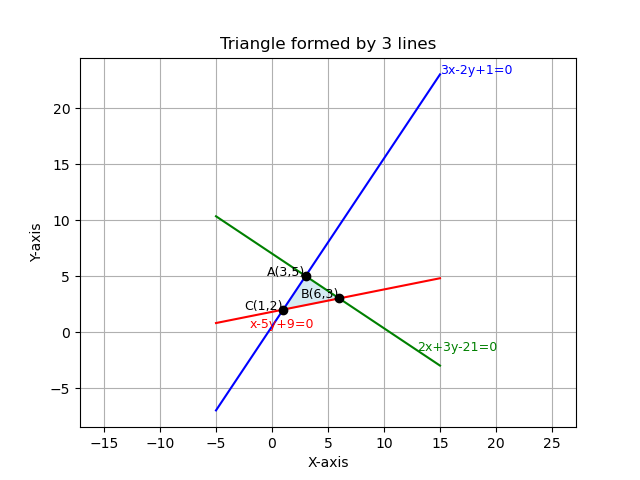
\includegraphics[width=0.9\columnwidth]{figs/fig8.png} 
\caption*{Fig: Representation of Triangle}
\label{Fig8}
\end{figure}

\end{document}
